\chapter{АНАЛИЗ ТЕКУЩИХ РЕШЕНИЙ ПОЛУЧЕНИЯ, АНАЛИЗА И ОБРАБОТКИ ЭКСПЕРТНОЙ ИНФОРМАЦИИ В ОБЛАСТИ ОБСЛУЖИВАНИЯ ПРОГРАММНОГО ОБЕСПЕЧЕНИЯ И ИНФОРМАЦИОННОЙ ИНФРАСТРУКТУРЫ} \label{chapt3}

\section{Обзор решений} \label{sect3_1}

\textbf{HP OpenView} \cite{HPOpenView} является комплексным программным решением по мониторингу ИТ инфраструктуры предприятия. Система имеет множество модулей. Данная система охватывает широкий спектр возможностей:
\begin{itemize}
	\item Мониторинг
	\item Регистрация инцидентов
	\item Управление системами
\end{itemize}
Система не поддерживает:
\begin{itemize}
	\item Понимание и формализация запросов
	\item Автоматическое исправление проблемы на основе формализации запроса
\end{itemize}


\begin{figure} [h] 
  \center
  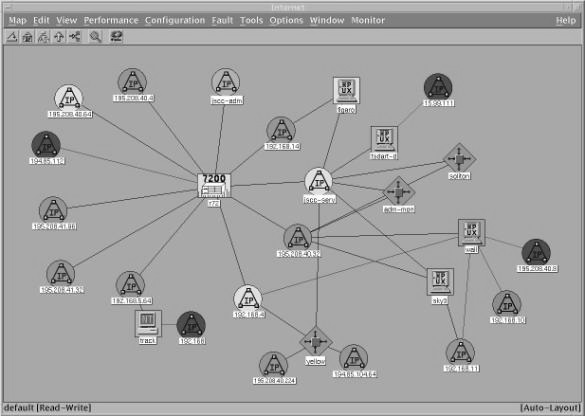
\includegraphics [scale=1.0] {hpopenview}
  \caption{HP OpenView} 
  \label{img:hpopenview}  
\end{figure}

\textbf{ServiceNOW} Средства автоматизации сервиса. Предоставляет следующие возможности:
\begin{itemize}
	\item Регистрация инцидентов
	\item Создание цепи обработки инцидента
\end{itemize}

Система не поддерживает:
\begin{itemize}
	\item Понимание и формализация запросов
	\item Автоматическое исправление проблемы на основе формализации запроса
\end{itemize}


\begin{figure} [h] 
  \center
  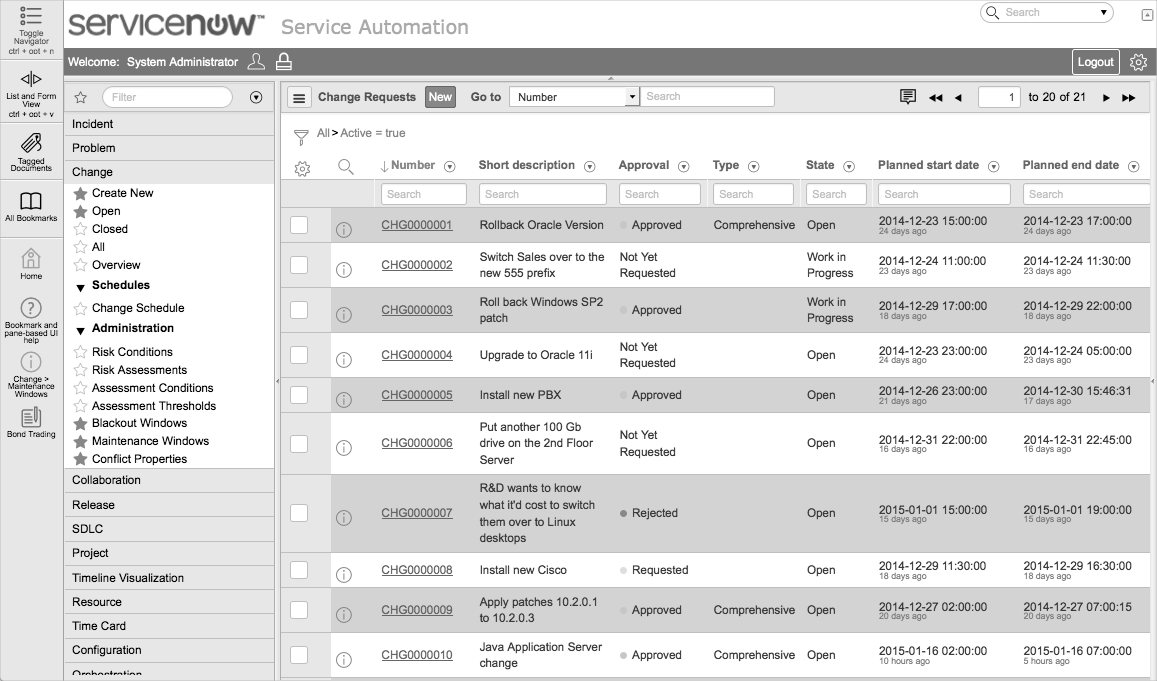
\includegraphics [scale=0.3] {svnow}
  \caption{Service NOW} 
  \label{img:svnow}  
\end{figure}

\textbf{IBMWatson} \ref{img:Watson-Analytics} Вопрос-ответная система поддерживает:
\begin{itemize}
	\item Понимания и формализацию запросов
	\item Поиск решений
\end{itemize}

Система не поддерживает:
\begin{itemize}
	\item Автоматическое исправление проблемы на основе формализации запроса
\end{itemize}


\begin{figure} [h] 
  \center
  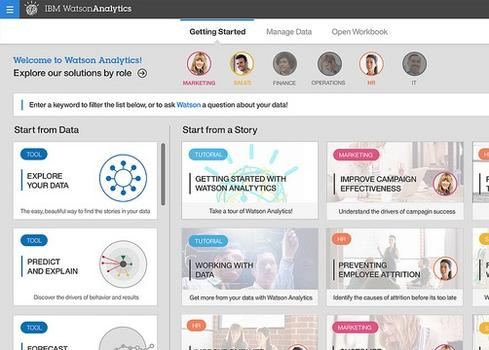
\includegraphics [scale=1.0] {Watson-Analytics}
  \caption{Пример работы системы Watson} 
  \label{img:Watson-Analytics}  
\end{figure}

\textbf{Прочие системы}
Кроме того существуют дополнительные способы автоматизации
\begin{itemize}
	\item Обработка инцидентов посредством регулярных выражений. В таком решение нет гибкости, так как обработка идет путем поиска ключевых слов вне контекста
	\item Обработка инцидентов при помощи скриптов. Автоматизирует лишь рутинные операции
\end{itemize}

\section{Требования к системе} \label{sect3_2}

Основными требованиями к системе является следующие:
\begin{itemize}
	\item Мониторинг
	\item Регистрация инцидентов
	\item Управление системами
	\item Создание цепи обработки (Workflow) инцидента
	\item Понимания и формализацию запросов на естественном языке
	\item Поиск решений
	\item Применение решений
	\item Обучение решению инцидента
	\item Умение проводить логические рассуждения: генерализацию, специализацию, синонимичный поиск
\end{itemize}

Требования к системе формировались исходя из возможностей специалистов поддержки, а также анализа проблем, которыми они занимаются. Большинство инцидентов тривиальные и типичные, но все они разные. Для человека проблема "Please insall Firefox" и "Please install Chrome" идентичные, но с точки зрения формализации - нет. Общее в них можно найти взглянув на генерализацию различающейся части. Firefox и Chrome являются пакетами программного обеспечения.

\subsection{Вывод по главе}
Все рассмотренные системы не соответствуют полному комплексу необходимых требований. В Таблице \ref{Comparsion} приведены сводные данные по системам.

\begin{longtable}{|p{6cm}|p{0.5cm}|p{0.5cm}|p{0.5cm}|}
 \caption[Сравнительный анализ существующих решений]{Сравнительный анализ существующих решений}\label{Comparsion} \\ 
 \hline
 
 \multicolumn{1}{|c|}{\textbf{Сравнительный пункт}} & \multicolumn{1}{c|}{\textbf{HP Open View}} & \multicolumn{1}{c|}{\textbf{ServiceNOW}} & \multicolumn{1}{c|}{\textbf{IBM Watson}} \\ \hline 
\endfirsthead
\multicolumn{2}{c}%
{{\bfseries \tablename\ \thetable{} -- продолжение}} \\
\hline \multicolumn{1}{|c|}{\textbf{Сравнительный пункт}} & \multicolumn{1}{c|}{\textbf{HP Open View}} & \multicolumn{1}{c|}{\textbf{ServiceNOW}} & \multicolumn{1}{c|}{\textbf{IBM Watson}}  \\ \hline 
\endhead

\hline \multicolumn{2}{|r|}{{Продолжение следует}} \\ \hline
\endfoot

\hline \hline
\endlastfoot
\hline
   Мониторинг & Да & Да & Да \\
   \hline
   Регистрация инцидентов & Да & Да & Да\\
   \hline
   Управление системами & Да & Нет & Нет \\
   \hline 
   Создание цепи обработки (Workflow) инцидента & Да & Да & Нет \\
   \hline 
   Понимания и формализацию запросов на естественном языке & Нет & Нет & Да \\
   \hline 
   Поиск решений & Нет & Нет & Да \\
   \hline 
   Применение решений & Нет & Нет & Нет \\
   \hline
   Обучение решению инцидента & Нет & Нет & Да \\
   \hline
   Умение проводить логические рассуждения: генерализацию, специализацию, синонимичный поиск & Нет & Нет & Нет \\
   \hline
   \textbf{Итоговые очки} & 4 & 3 & 5 \\
   \hline 
\end{longtable}


\clearpage